\section{Strong-field Kerr orbits, photon spheres, and static-mesh clusters}\label{sec:kerr}

Strong-field trajectories around stationary Kerr black holes (up to near-extremal dimensionless spin) and dynamical vacuum puncture mergers benchmark fourth-order symplectic time integration, unified massive and null geodesics, $C^2$ quintic spatial metric reconstruction, and kinetic distributional fidelity from single tracers up to $N = 10^5$ packets.

\subsection{Sheared Kerr cloud and compute-error Pareto frontier}\label{sec:kerr_pareto}

A warm spherical kinetic cloud centered at $\bm{x}_0 = (6.0, 0.0, 1.5)\,M$ with coordinate radius $M$, inclined prograde boost grazing $r_{\min} \approx 1.7\,M > r_+$, and isotropic momentum spread $\sigma_u = 0.06$ tests differential shearing in analytic Cartesian Kerr--Schild geometry ($a = 0.9\,M$) through $t = 30\,M$ against a $10^5$-particle Monte Carlo reference.

\begin{figure}[tbp]
\centering
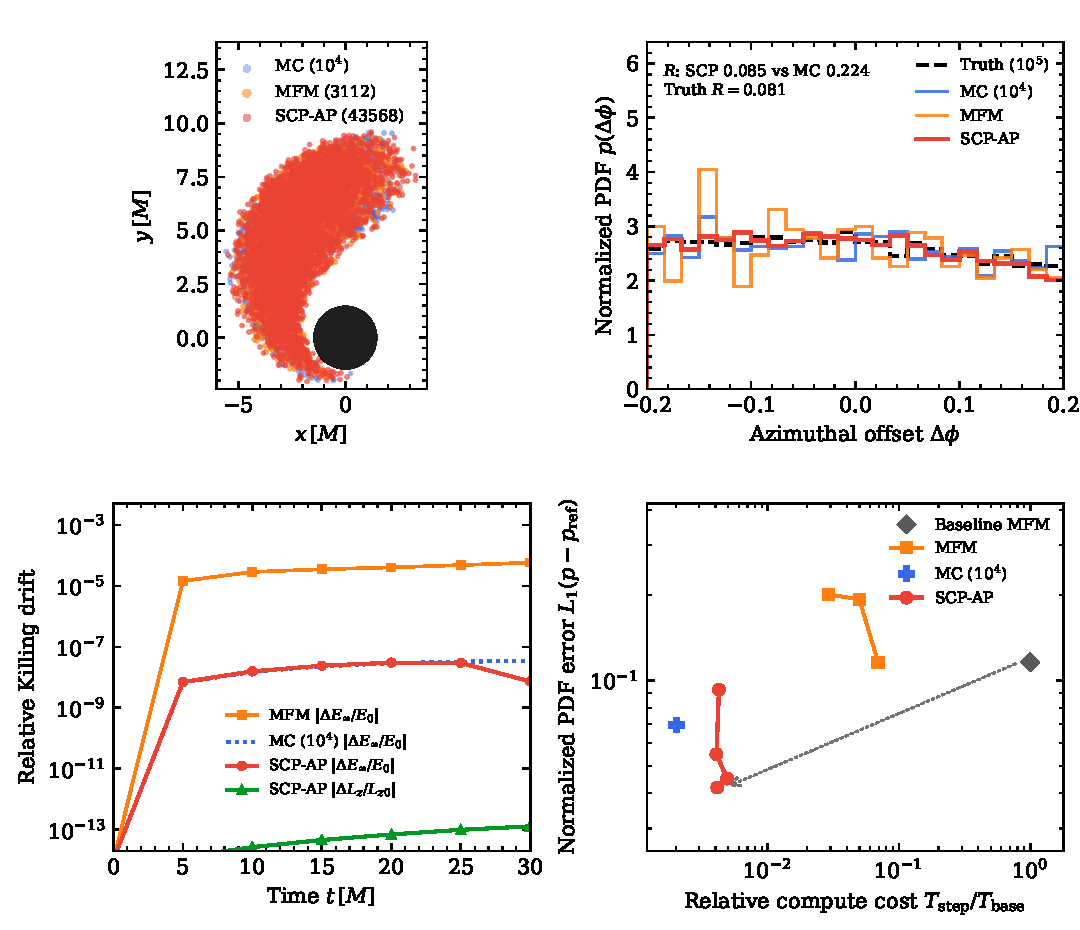
\includegraphics[width=\columnwidth]{figures/fig_kerr_pareto_arc.pdf}
\caption{\label{fig:kerr_pareto_arc}%
Sheared Kerr ($a = 0.9\,M$) cloud at $t = 30\,M$ for continuum MFM, Monte Carlo PIC ($10^4$), and fifth-degree Stroud cubature packets ($43568$) outside $r_+$. Top right: Azimuthal density profile vs $10^5$ reference. Bottom: Killing invariant drifts and compute-error Pareto frontier.}
\end{figure}

In Fig.~\ref{fig:kerr_pareto_arc}, continuum MFM exhibits azimuthal roughness and secular Killing-energy and angular-momentum drift driven by neighbor-element gradient diffusion across strongly sheared neighbors. Expanding initialized velocity bases into fifth-degree Stroud cubature packets eliminates inter-element shear diffusion, tracks the $10^5$-particle azimuthal distribution smoothly, bounds stationary Killing drifts near machine precision, and occupies the dominant lower-left corner of the Pareto frontier roughly two orders of magnitude faster than continuum MFM while running ahead of equal-cost Monte Carlo sampling.

\subsection{Fourth-order zoom-whirl passages, null light rings, and merger tracers}\label{sec:kerr_gl4}

Highly eccentric strong-field passages, critical null rays, and dynamical binary mergers separate temporal integration accuracy from spatial metric discretization error. Following Ref.~\cite{Wu:2026nrpic}, we first benchmark an eccentric ($e = 0.99$) inclined Kerr ($a = 0.9\,M$) passage reaching pericenter $r_{\min} \approx 2.1\,M$ over $t \in [0, 230]\,M$ across spherical Kerr--Schild, Cartesian Kerr--Schild, and finite-difference lattice metrics ($\Delta x = M/40$), alongside a $t = 600\,M$ inclined torus on a six-level static refinement hierarchy (finest spacing $0.25\,M$). As shown in Figs.~\ref{fig:gl4_kerr_clusters} and~\ref{fig:physics_kerr_single_particle}, fourth-order \texttt{GL4} integration cuts $e = 0.99$ energy and Carter-constant drifts by roughly six orders of magnitude compared to implicit midpoint integration and reduces final position separation relative to an eighth-order Dormand--Prince reference down to sub-micrometer scales (with complete benchmark digits compiled in Appendix Table~\ref{tab:bench_kerr_orbits}). Nonuniform-step tests confirm the theoretical third-order temporal metric convergence ($p \approx 3.0$) of three-level quadratic Lagrange time interpolation versus second-order linear blending. On evolved dynamical Z4c single-puncture and head-on binary black hole mergers ($x_0 = \pm 5\,M$, merging near $t \approx 50\,M$), \texttt{GL4} tracers preserve axial momentum and equatorial reflection symmetry cleanly while resolving polar accretion.

\begin{figure*}[tbp]
\centering
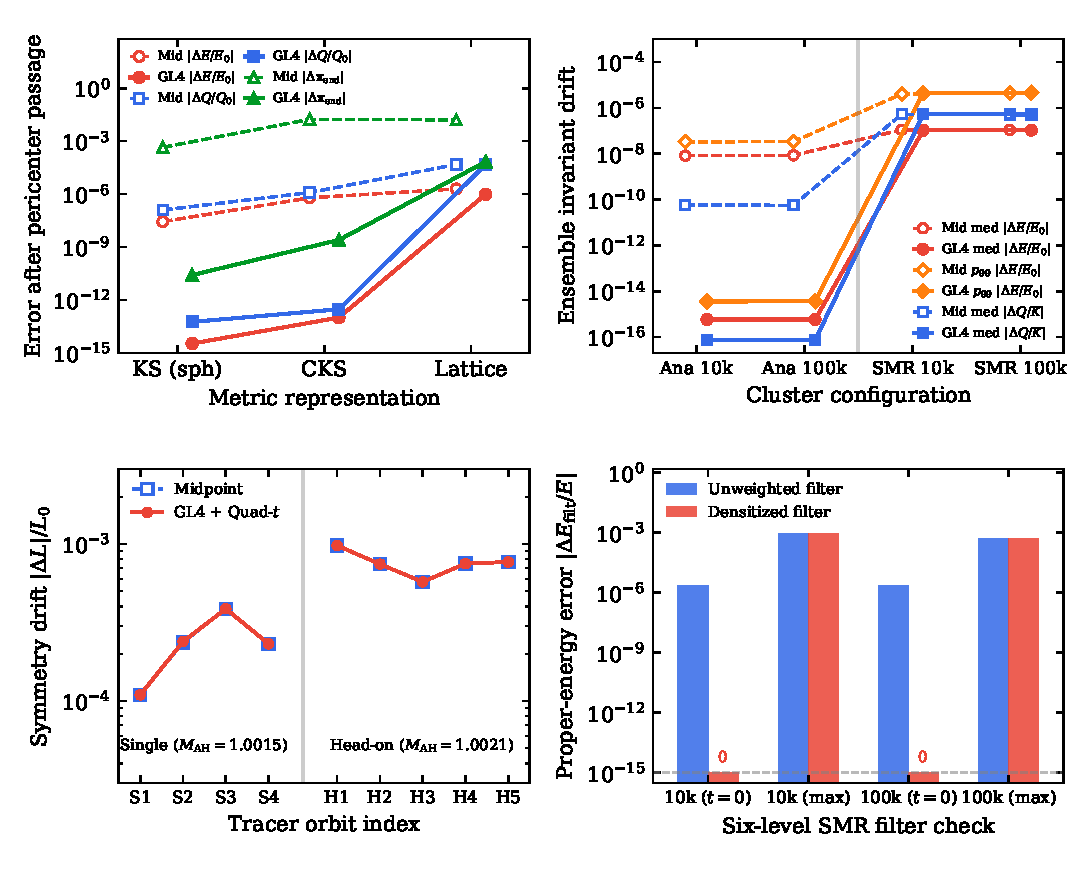
\includegraphics[width=\textwidth]{figures/fig_gl4_kerr_clusters.pdf}
\caption{\label{fig:gl4_kerr_clusters}%
Strong-field integrator accuracy across Kerr ($a=0.9\,M$) geodesics and six-level static-mesh clusters ($t = 200\,M$, $N = 10^4, 10^5$). Top: Energy, Carter constant $Q$, and endpoint position errors after $e = 0.99$ pericenter passage plus median cluster drifts. Bottom: Nonuniform-step metric time-interpolation scaling and dynamical puncture merger invariants.}
\end{figure*}

\begin{figure*}[tbp]
\centering
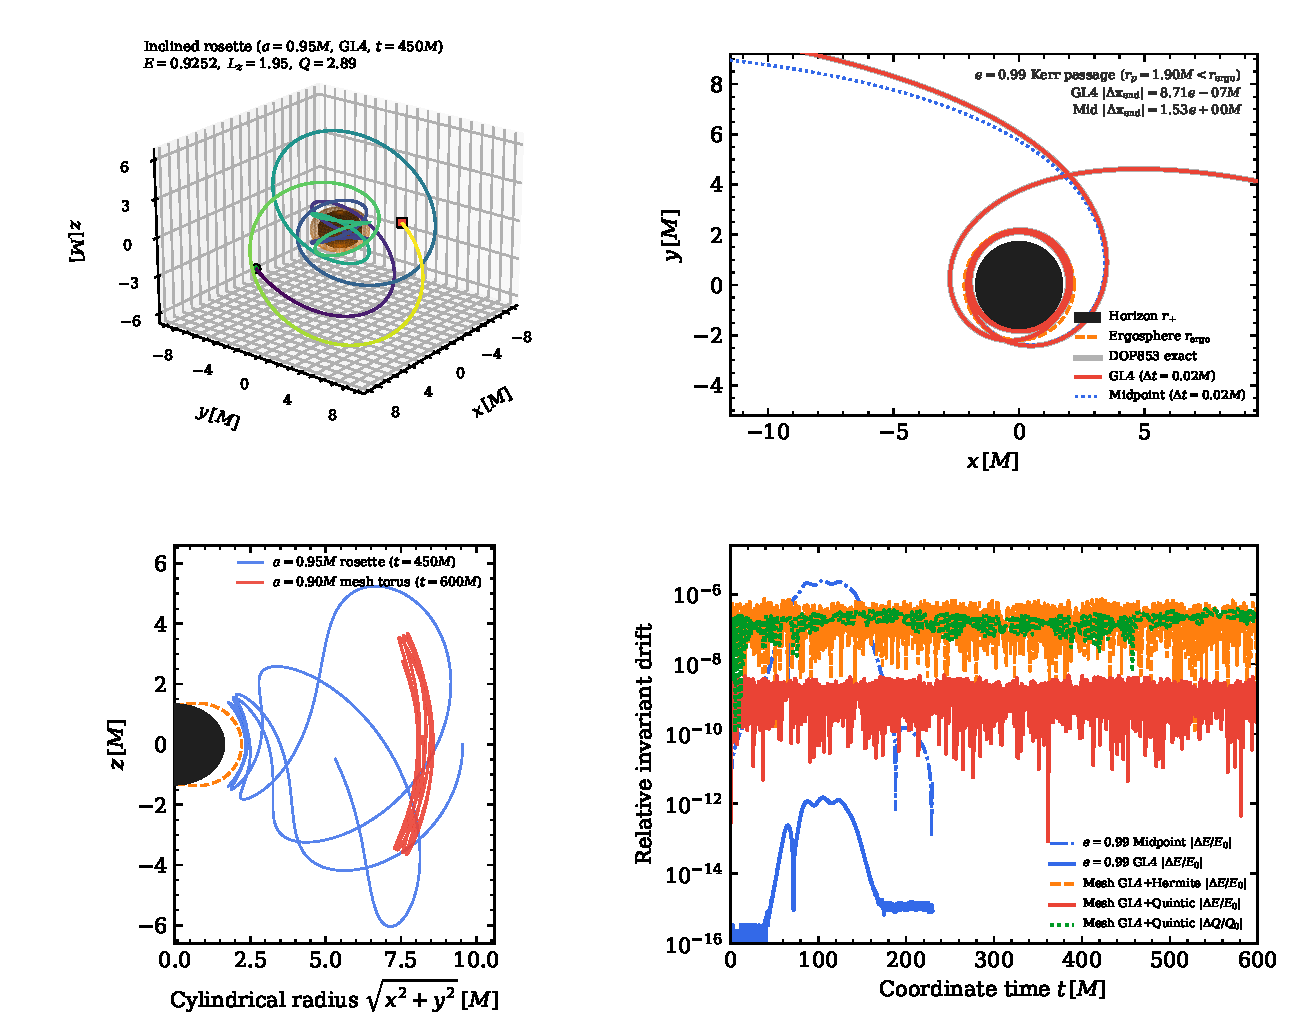
\includegraphics[width=\textwidth]{figures/fig_physics_kerr_single_particle.pdf}
\caption{\label{fig:physics_kerr_single_particle}%
Single-particle Kerr geodesic verification. Top left: Three-dimensional inclined rosette ($a = 0.95\,M$, \texttt{GL4}, $t = 450\,M$) outside $r_+$ and the ergosphere. Top right: $e = 0.99$ passage ($a = 0.90\,M$, $\Delta t = 0.02\,M$) comparing \texttt{GL4} and midpoint vs eighth-order reference. Bottom: Meridional envelopes and invariant drift histories.}
\end{figure*}

\begin{figure*}[tbp]
\centering
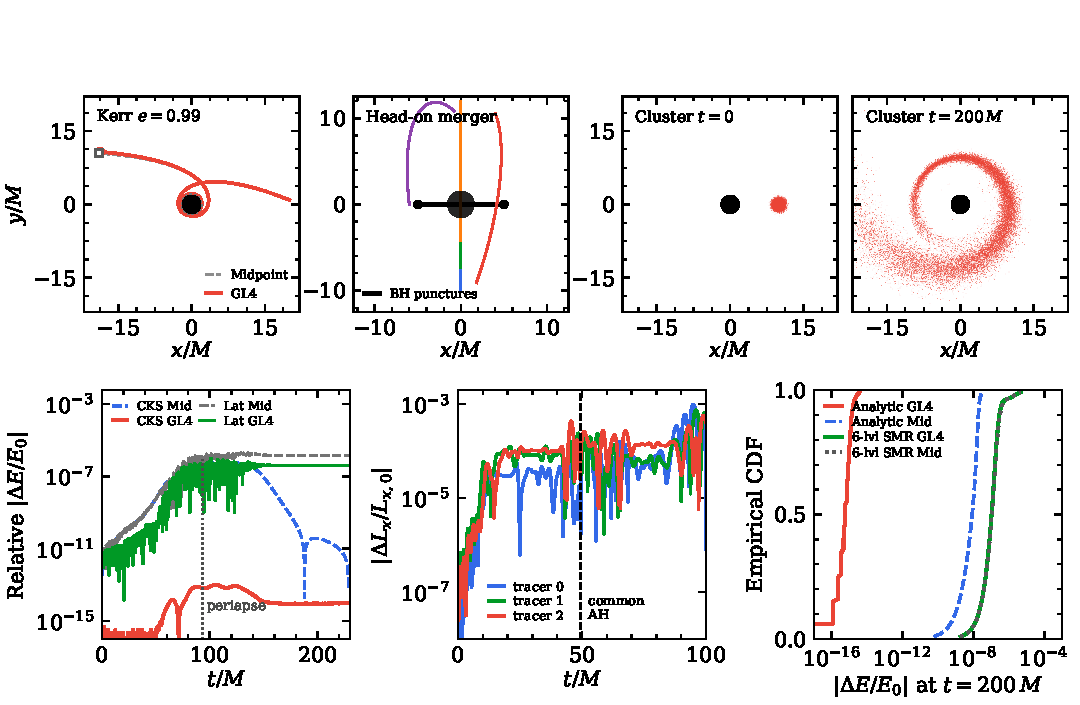
\includegraphics[width=\textwidth]{figures/fig_physics_kerr_cluster_orbits.pdf}
\caption{\label{fig:physics_kerr_cluster_orbits}%
Equatorial orbit portraits and invariant distributions. Top: $a = 0.9\,M$, $e = 0.99$ passage, dynamical Z4c head-on binary merger punctures and tracers, and $N = 10^5$ six-level static-mesh Kerr cluster winding ($t = 0$ to $200\,M$). Bottom: Pericenter energy drift, head-on tracer angular momentum error, and cluster energy empirical CDFs.}
\end{figure*}

Pushing closer to extremality tests both ergospheric frame dragging and spatial metric reconstruction in extreme curvature gradients. Figure~\ref{fig:physics_kerr_a0999_e0999} examines a near-extremal Kerr black hole across three orbits: an inclined ($25^\circ$) high-eccentricity ($e \to 1$, tabulated in Appendix Table~\ref{tab:bench_kerr_orbits}) pericenter passage dipping inside the ergosphere ($r_{\rm p} = 1.35\,M < r_{\rm ergo} = 2.00\,M$, hovering just outside the event horizon $r_+$) through more than four azimuthal whirls; a $t = 450\,M$, $40^\circ$-inclined bound zoom-whirl rosette ($r_{\rm p} = 1.55\,M$, $r_{\rm a} = 9.5\,M$); and a $t = 500\,M$ static-mesh inclined torus ($n_g = 4$). Along the four-whirl encounter at $\Delta t = 0.02\,M$, both baseline second-order pushers (implicit midpoint and symmetric-gauge spacetime Boris) incur secular orbit-phase errors exceeding five orders of magnitude above \texttt{GL4}, which preserves geodesic energy to twelve digits and Carter constant to eleven digits while matching the eighth-order trajectory closely. On the static mesh ($\Delta x = 0.25\,M$), replacing four-point cubic Hermite with $C^2$ six-node quintic Hermite reduces mesh-limited energy and Carter drifts by roughly two orders of magnitude (Table~\ref{tab:bench_kerr_orbits}).

\begin{figure*}[tbp]
\centering
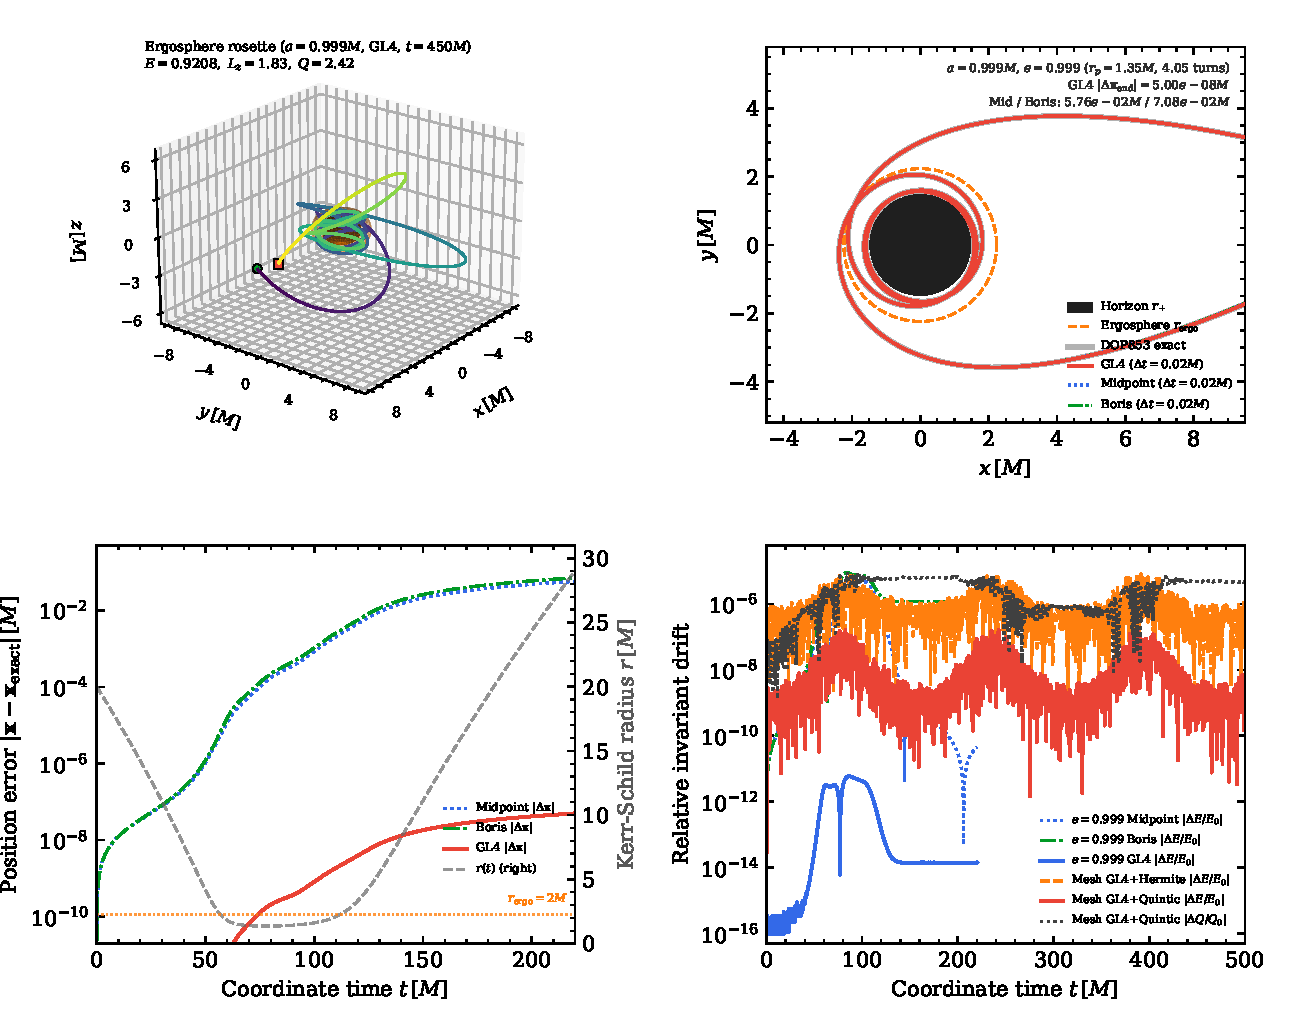
\includegraphics[width=\textwidth]{figures/fig_physics_kerr_a0999_e0999.pdf}
\caption{\label{fig:physics_kerr_a0999_e0999}%
Near-extremal Kerr ($a = 0.999\,M$) zoom-whirl geodesics. Top left: $3$D inclined bound rosette ($t = 450\,M$) diving deep inside the ergosphere outside $r_+$. Top right: $e = 0.999$ four-whirl passage comparing \texttt{GL4}, midpoint, and Boris vs eighth-order reference. Bottom: Energy and position error growth plus static-mesh quintic vs cubic Hermite torus drifts.}
\end{figure*}

Setting $\varepsilon = 0$ activates null geodesic transport inside identical pusher kernels. Figure~\ref{fig:physics_kerr_a090_lightring} probes the unstable photon-sphere separatrix of an $a = 0.90\,M$ Kerr black hole across $32$ equatorial rays straddling the prograde critical impact parameter $\xi_{c,+}$ at the prograde light ring $r_{\rm ph}^+$, perched prograde and retrograde light-ring photons, and a bound $3$D inclined spherical photon-shell orbit at $r_{\rm sph} = 2.2\,M$. Across eight decades of impact-parameter detuning $\delta\xi/\xi_{c,+}$, \texttt{GL4} reproduces the exact prograde Lyapunov winding slope (close to one azimuthal turn per decade of tuning) cleanly down to $\delta\xi/\xi_{c,+} = 10^{-8}$, whereas implicit midpoint integration prematurely destabilizes and undercounts light-ring turns even at tight step size. For perched prograde photons, \texttt{GL4} nearly triples the dwell orbit count before roundoff growth drives radial departure ($8.95$ vs $3.40$ orbits at $\Delta t = 0.02\,M$).

\begin{figure*}[tbp]
\centering
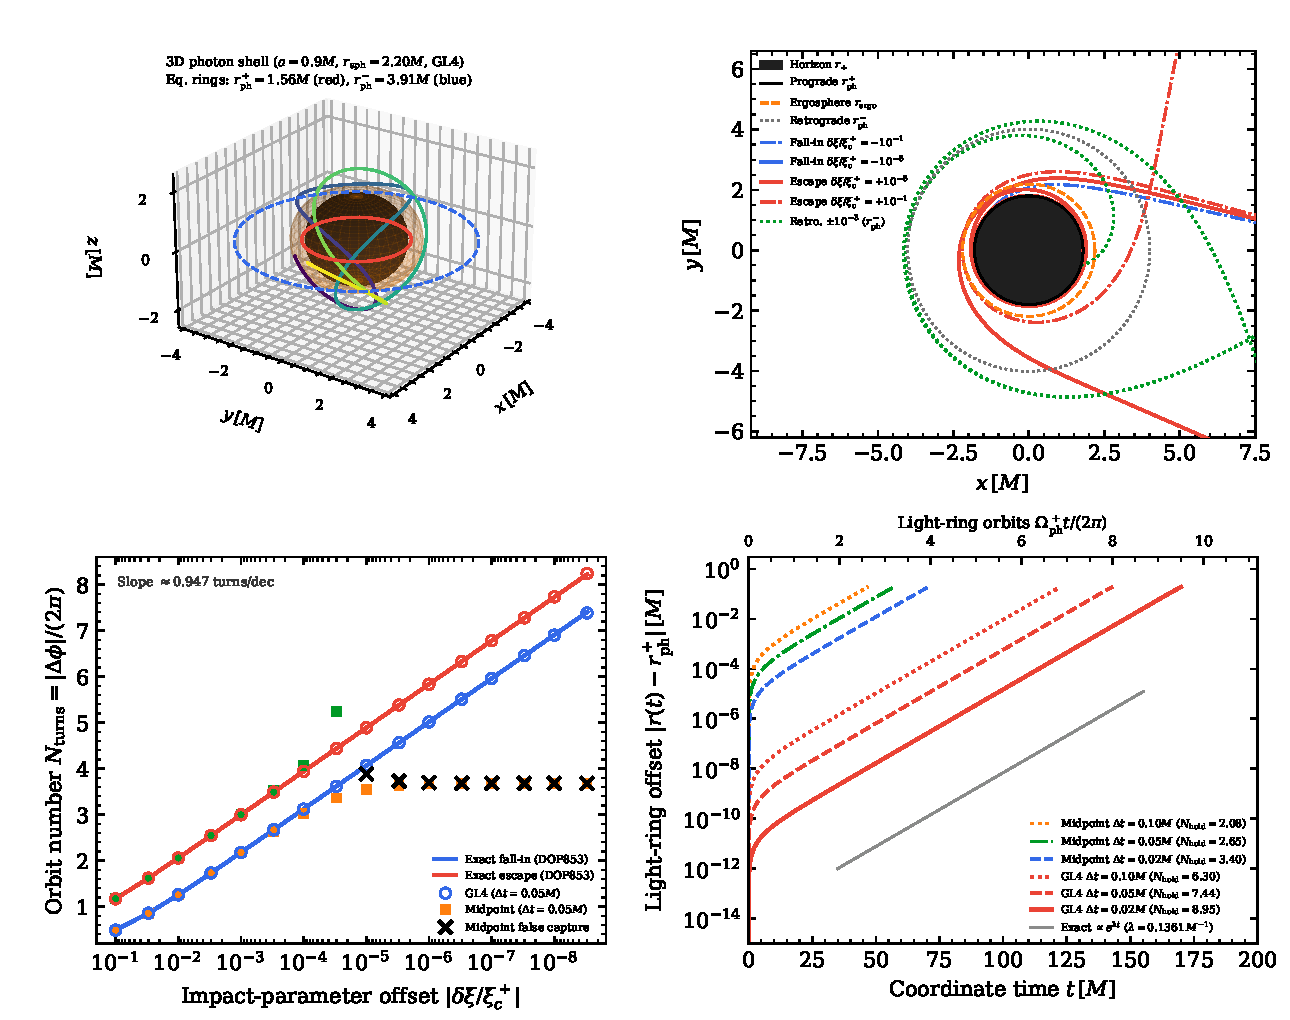
\includegraphics[width=\textwidth]{figures/fig_physics_kerr_a090_lightring.pdf}
\caption{\label{fig:physics_kerr_a090_lightring}%
Kerr ($a = 0.90\,M$) null light-ring separatrix ($\varepsilon = 0$). Top left: Plunging and escaping rays straddling $\xi_{c,+}$ around $r_{\rm ph}^+ = 1.558\,M$. Top right: Fall-in orbit count $N_{\rm turns}$ vs impact-parameter detuning $|\delta\xi|/\xi_{c,+}$, tracking the theoretical Lyapunov slope. Bottom: $3$D inclined photon-shell orbit ($r_{\rm sph} = 2.20\,M$) and perched light-ring stability.}
\end{figure*}

\subsection{Breaking the spatial error floor and four-regime orbit comparison}\label{sec:kerr_quintic_cmp}

On six-level static-mesh Kerr clusters of $N = 10^4\text{--}10^5$ bound orbits evolved to $t = 200\,M$ (Fig.~\ref{fig:physics_kerr_cluster_orbits}, top-right and bottom-right panels), \texttt{GL4} integration lowers analytic invariant drift to machine precision while smoothly phase-mixing the localized ensemble into a differentially wound torus. Under standard four-point cubic Hermite interpolation on the mesh metric, however, both second-order and fourth-order pushers stall identically along an empirical cumulative distribution floor near $|\Delta\Egeo/\Egeo|_{\rm med} \approx 10^{-7}$, set by the $\mathcal{O}(h^3)$ gradient discontinuity across cell faces.

\begin{figure*}[tbp]
\centering
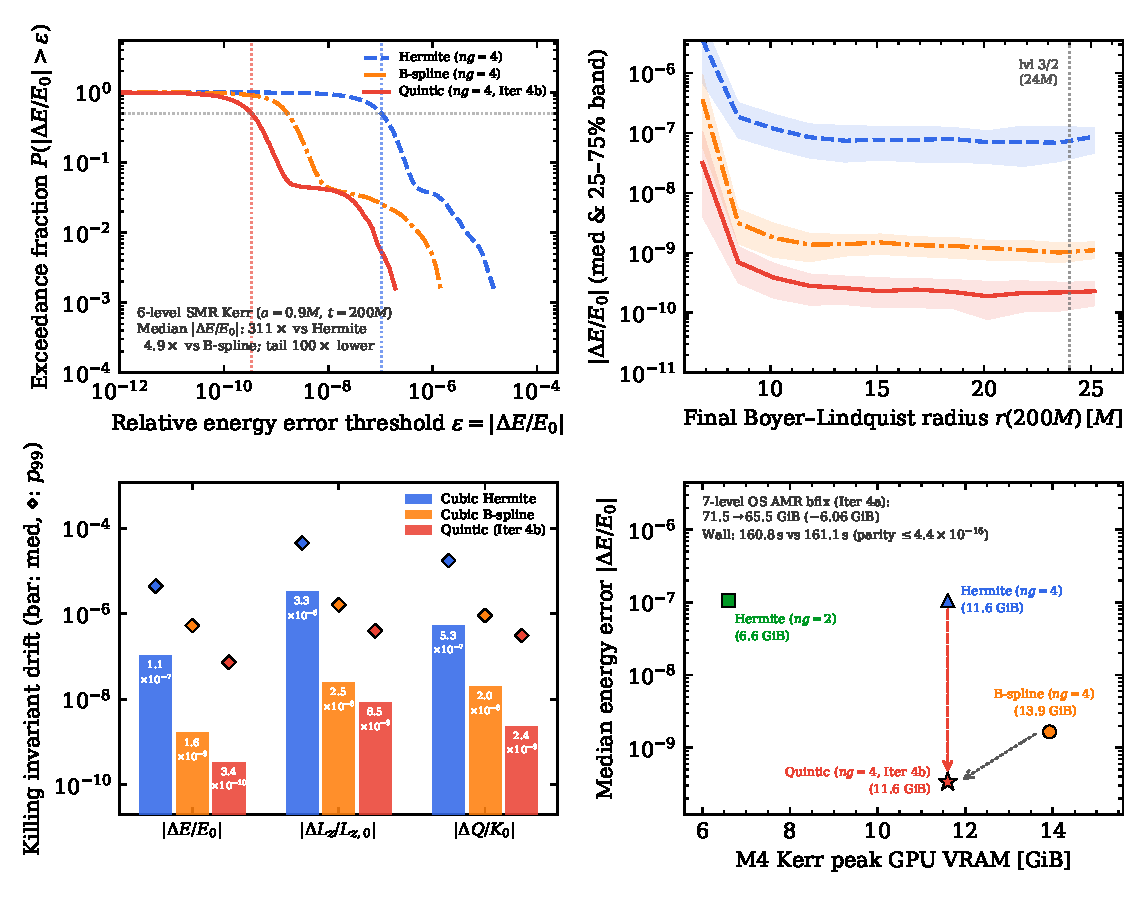
\includegraphics[width=\textwidth]{figures/fig_iter4_quintic_kerr_diagnostics.pdf}
\caption{\label{fig:iter4_quintic_kerr}%
Eliminating the six-level static-mesh Kerr ($a = 0.9\,M$, $N = 10^4$, $t = 200\,M$) spatial error floor with zero-overhead $C^2$ quintic Hermite reconstruction and boundary-only refluxing. Top: Empirical CCDF and radial scaling of $|\Delta\Egeo/\Egeo|$ vs cubic Hermite and cubic B-splines. Bottom: Median invariant drifts and device-memory footprint across Kerr SMR and Oppenheimer--Snyder AMR.}
\end{figure*}

Replacing the four-point cubic stencil with zero-overhead $C^2$ six-node quintic Hermite reconstruction breaks this spatial floor completely without allocating auxiliary spline coefficient arrays (Fig.~\ref{fig:iter4_quintic_kerr}). Across all $10^4$ orbits on the six-level hierarchy, $C^2$ quintic interpolation reduces median energy drift by more than two orders of magnitude relative to cubic Hermite (outperforming sharpened cubic B-splines nearly fivefold while saving over $2.3\,\mathrm{GiB}$ of device memory), cuts axial angular-momentum and Carter errors comparably, preserves cluster phase-mixing coherence identically, and holds conservative filter mass drift near $10^{-15}$. Simultaneously replacing three directional conservative filter sweeps per pass with the unsplit seven-point harmonic active-block filter cuts inter-block synchronization threefold and lowers $t = 200\,M$ Kerr runtime up to threefold without altering any orbit invariant (Table~\ref{tab:bench_speed_memory}).

\begin{figure*}[tbp]
\centering
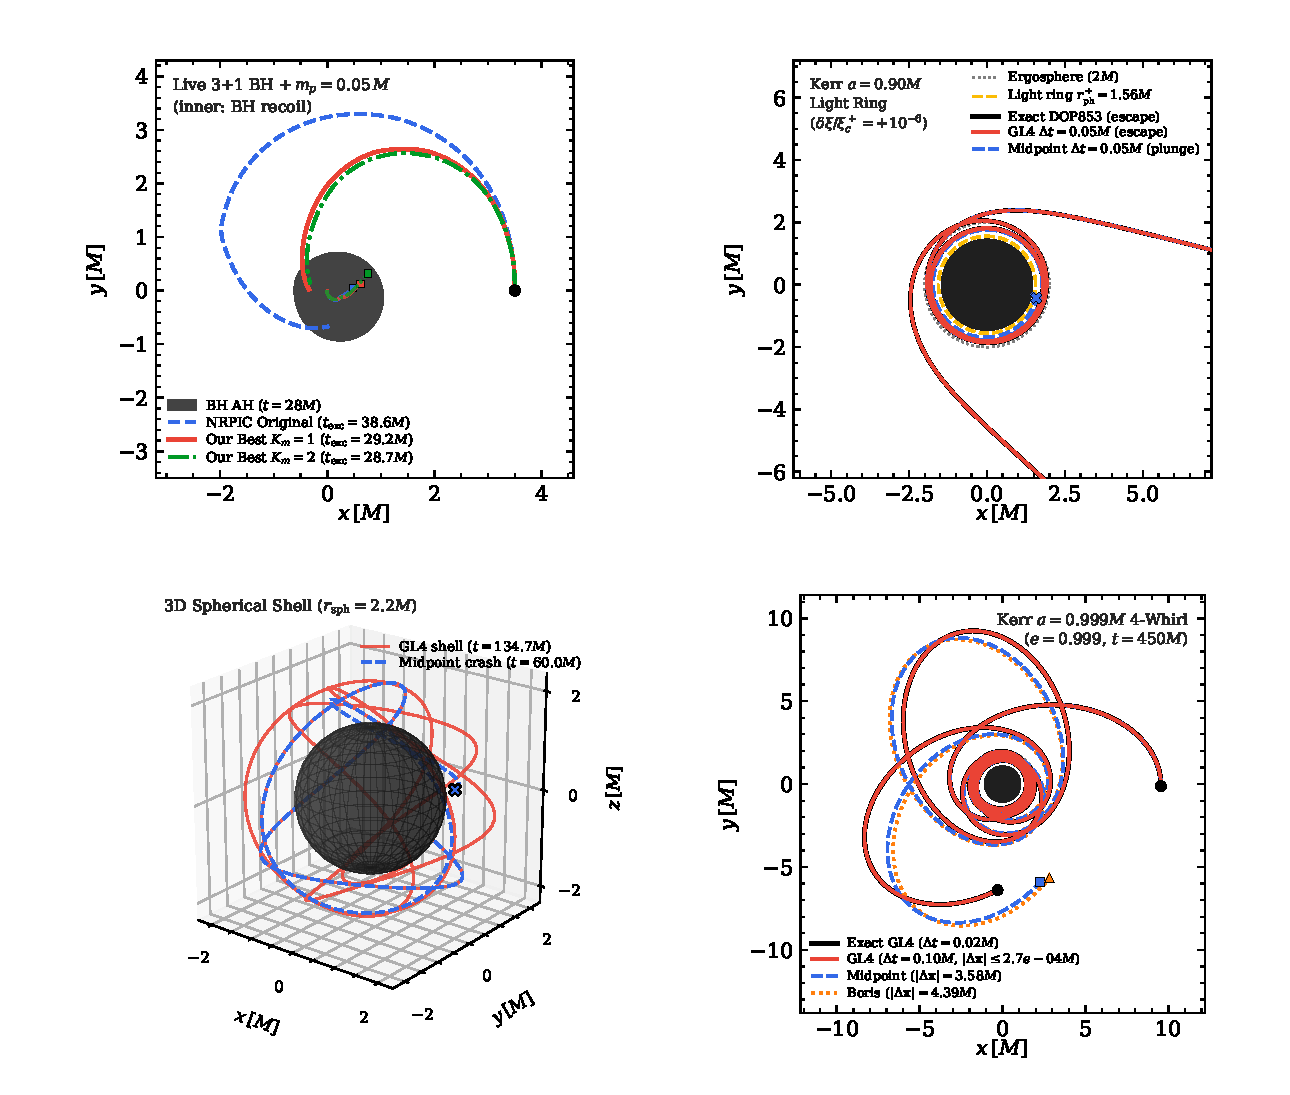
\includegraphics[width=\textwidth]{figures/fig_compare_orig_vs_best_orbits.pdf}
\caption{\label{fig:compare_orig_vs_best_orbits}%
Physical trajectory comparison between baseline second-order NRPIC (dashed) and the high-order metric-conservative solver (solid) across four strong-field regimes: (top left) dynamical $3+1$ spinning-puncture inspiral ($q = 0.05$); (top right) Kerr $a=0.9\,M$ photon separatrix ($\delta\xi/\xi_{c,+}=+10^{-6}$); (bottom left) $3$D inclined $r_{\rm sph}=2.2\,M$ photon shell; (bottom right) coarse-step $a=0.999\,M$ four-whirl encounter.}
\end{figure*}

Figure~\ref{fig:compare_orig_vs_best_orbits} translates these numerical gains directly into physical trajectory fidelity across four strong-field regimes. In dynamical $3+1$ black hole back-reaction ($q = 0.05$, Sec.~\ref{sec:collapse_backreaction}), plain-filter energy leakage delays baseline plunge by nearly $10\,M$; on the $a = 0.90\,M$ prograde photon separatrix at $\delta\xi/\xi_{c,+} = +10^{-6}$, baseline midpoint prematurely plunges after $3.7$ whirls whereas \texttt{GL4} captures $5.8$ tight light-ring whirls before escaping cleanly along the exact reference geodesic; on the $3$D spherical photon shell ($r_{\rm sph} = 2.2\,M$), \texttt{GL4} holds the precessing bound shell past $t = 134\,M$ while baseline midpoint plunges at $t = 60\,M$; and along a coarse-step ($\Delta t = 0.1\,M$) near-extremal four-whirl passage, \texttt{GL4} tracks the exact phase down to sub-milliradian error while both baseline midpoint and DGREM Boris accumulate macroscopic dephasing.
